\section{Osmosi}

Consideriamo una membrana posta tra due compartimenti contenenti l'uno una soluzione e l'altro un puro solvente, ad esempio acqua, come schematizzato in \figurename~\ref{osmosi}a.
\begin{figure}[htb]
	\centering
		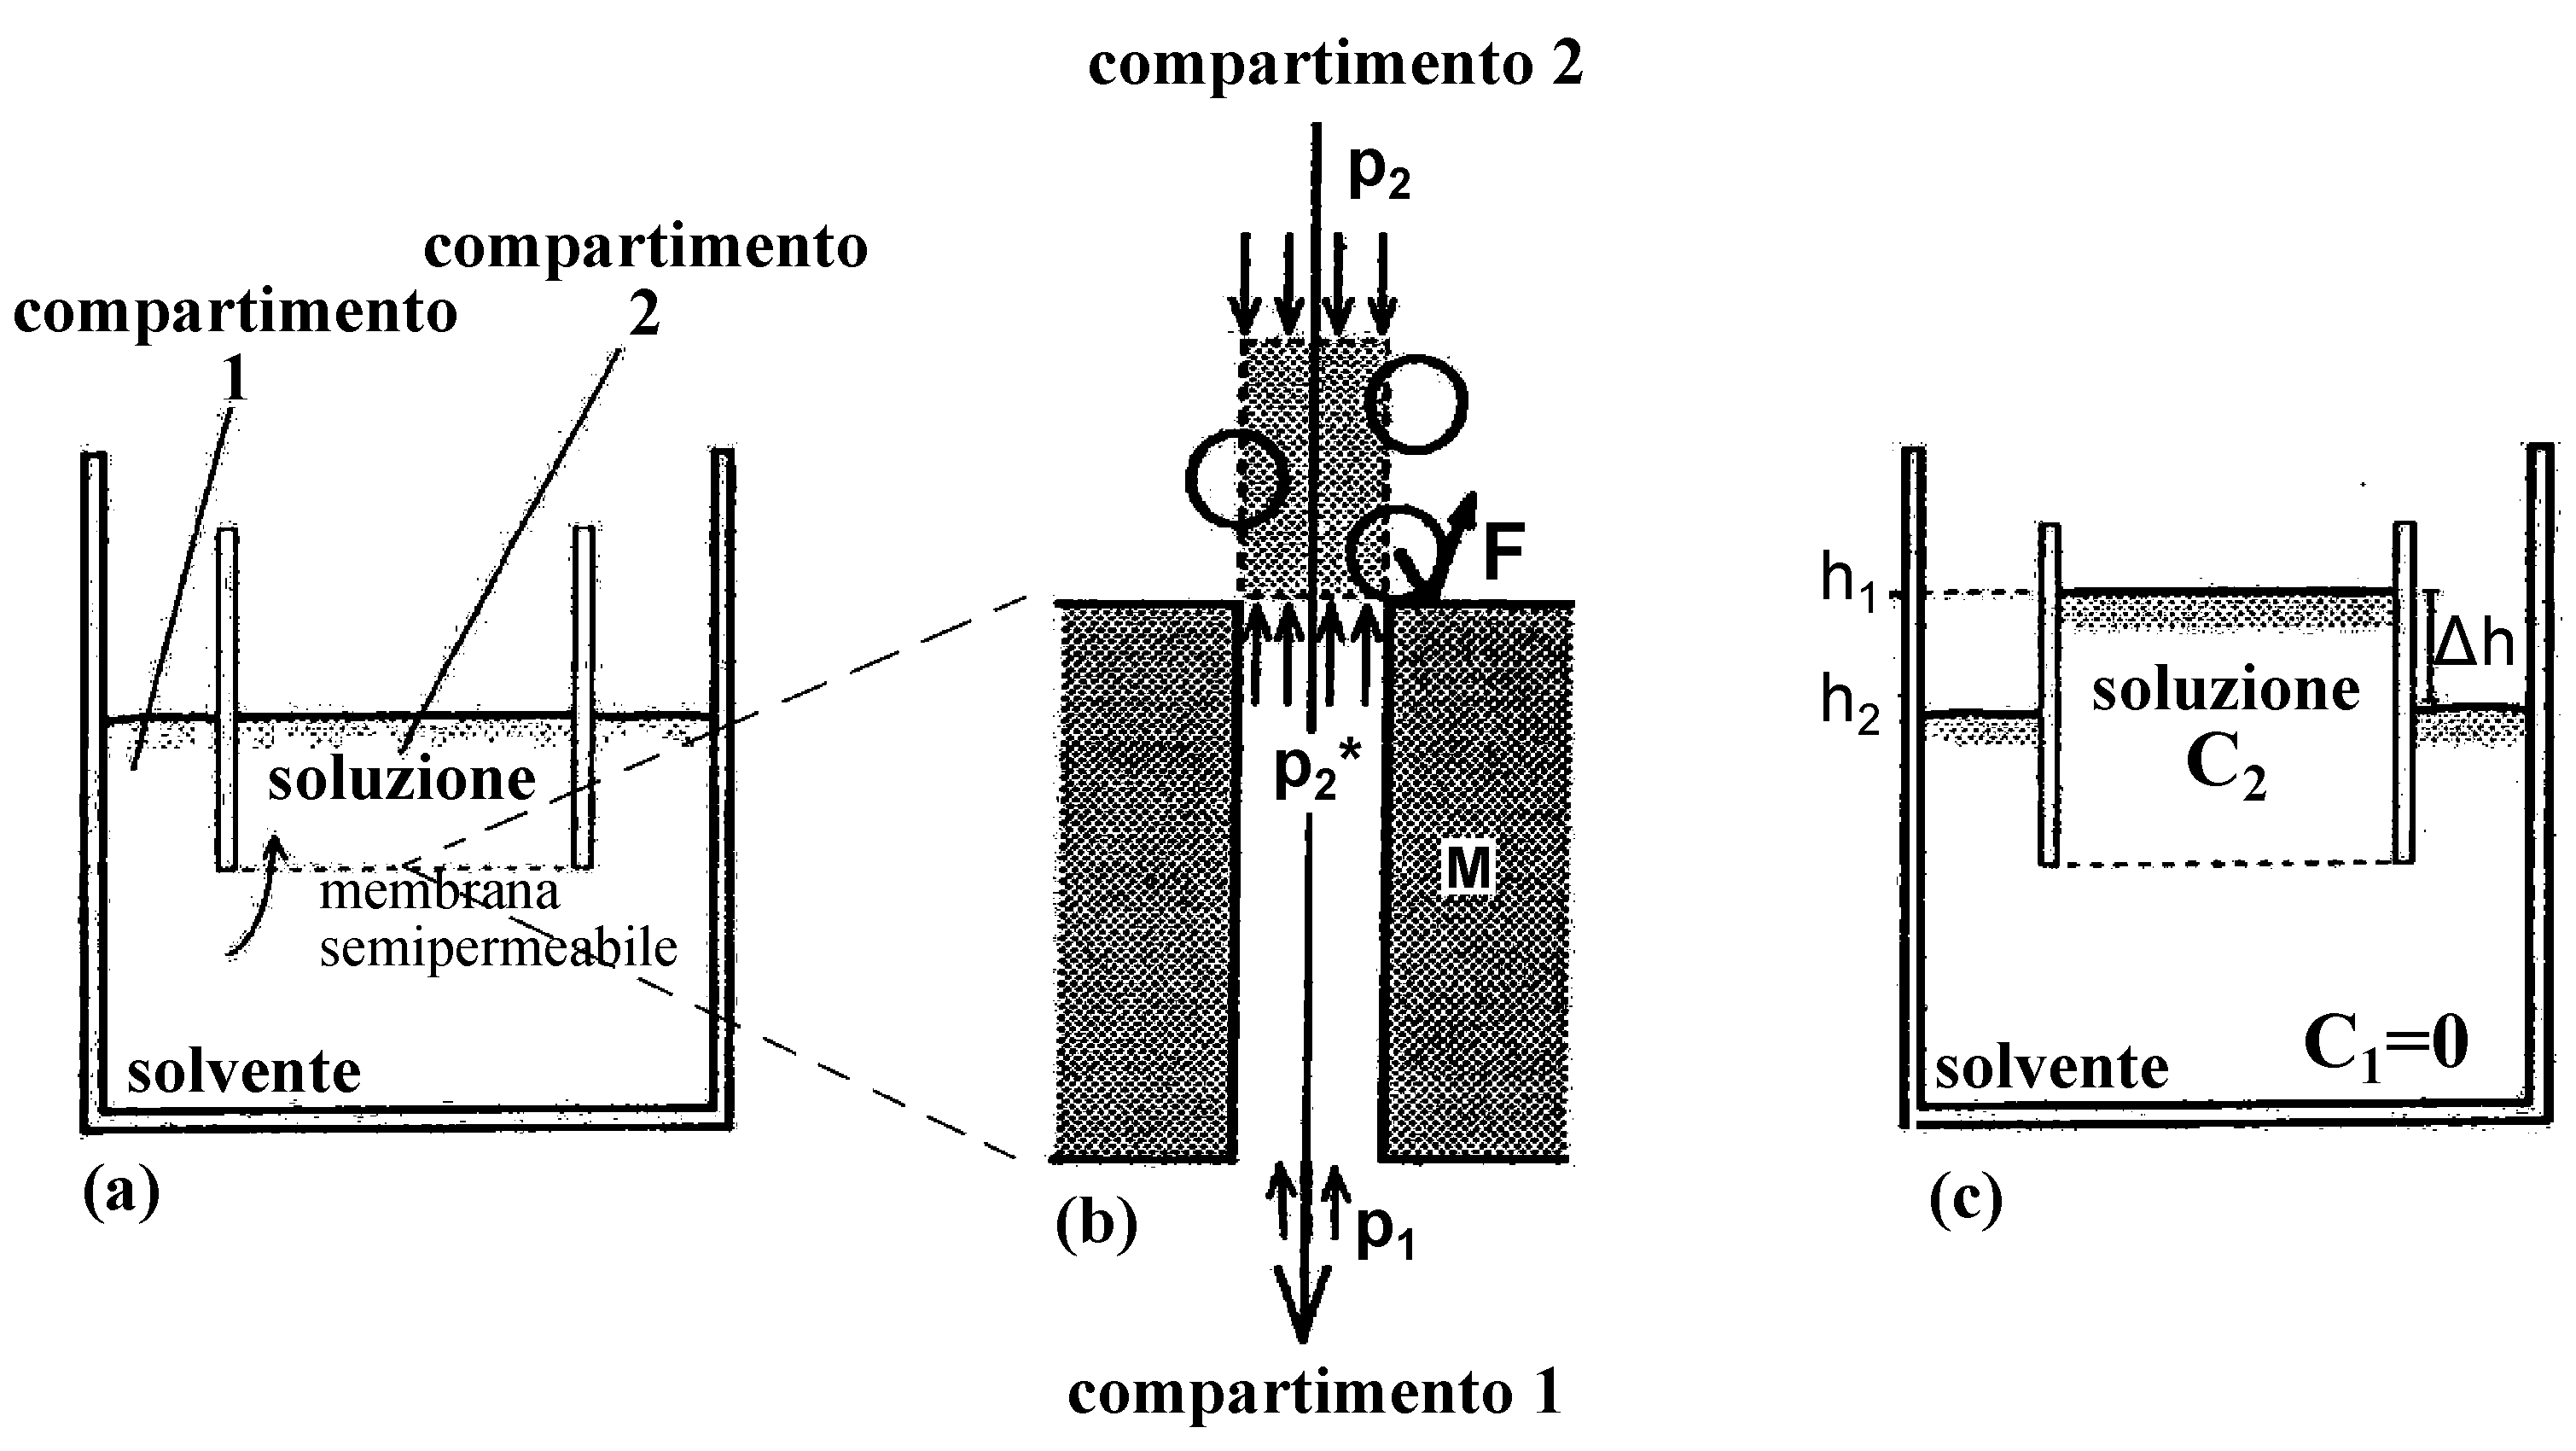
\includegraphics[width=\textwidth]{immagini/osmosi.eps}
		\caption{Il fenomeno dell'osmosi: (a) i due compartimenti sono a contatto tramite una membrana semipermeabile attraverso cui fluisce il solvente; (b) le molecole di soluto rimbalzano sulla membrana provocando una diminuizione di pressione all'imbocco del poro; (c) il livello del compartimento del soluto si alza fino a che la pressione idrostatica equilibra quella osmotica.}\label{osmosi}
\end{figure}
\noindent
Se i pori della membrana hanno dimensioni tali da lasciar passare il solvente ma non il soluto, questo non potrà diffondere da un compartimento all'altro e la membrana si dirà \textit{semipermeabile} al soluto. Nonostante non agisca alcuna pressione idrostatica, dopo un po' di tempo si osserva un innalzamento del livello della soluzione fino a una nuova posizione di equilibrio (\figurename~\ref{osmosi}c). L'innalzamento è tanto maggiore quanto più elevata è la concentrazione del soluto nel compartimento~2. Questo fenomeno è chiamato \textit{osmosi}. Possiamo comprendere l'osmosi facendo alcune considerazioni fenomenologiche sulle forze che agiscono sulle molecole. Inizialmente le pressioni idrauliche ai due lati della membrana si equivalgono. Le molecole di soluto nel compartimento~2 non riescono a passare la membrana perché hanno dimensione maggiore di quella dei pori, e quindi rimbalzano sul bordo dei pori muovendosi in verso opposto a quello del gradiente di concentrazione. In \textit{prossimità} dei pori questo moto unidirezionale delle molecole di soluto (\figurename~\ref{osmosi}b) trascina con se, per attrito viscoso, le molecole di solvente dall'interno dei pori verso il compartimento~2, creando all'interno dei pori una pressione idraulica $p_2^*<p_2$. Quindi ora, dato che $p_1 = p_2 > p_2^*$, si crea un flusso di solvente dal compartimento~1 verso il compartimento~2. Questo flusso di solvente si evidenzia tramite una ``pressione efficace'' poiché, nella situazione finale, i suoi effetti sono bilanciati dalla pressione idrostatica determinata dal dislivello $\Delta h$. A questa pressione di richiamo di solvente, che ha \textit{vettorialmente}\footnote{è importante ricordarsi di ciò nel momento in cui si fanno i bilanci pressori come nell'equazione~\ref{Qtpi}: la pressione idraulica è una pressione di \textit{spinta} e il fluido si muove verso le pressioni idrauliche minori; la pressione osmotica è una pressione di \textit{risucchio} e il fluido si muove verso le pressioni osmotiche maggiori.} lo stesso verso del gradiente di concentrazione del soluto, si dà il nome di \textit{pressione osmotica} e si indica con la lettera $\Pi$.
Per soluzioni diluite vale la seguente relazione, analoga a quella per i gas perfetti, stabilita da \textit{Van't Hoff}:
\begin{equation}\label{vhoff}
	\Pi V = \delta n R T
\end{equation}
dove $\delta$ è il coefficiente di dissociazione elettrolitica, pari a uno se il soluto non si dissocia\footnote{per una mole di $NaCl$, $\delta=2$ perché questo composto, in soluzione, si dissocia in due moli: una mole di $Na^+$ e una mole di $Cl^-$.}, $n$ è il numero di moli del soluto, $R$ è la costante dei gas perfetti e $T$ la temperatura assoluta del sistema. La pressione osmotica complessiva di una soluzione contenente più soluti è data dalla somma delle pressioni osmotiche parziali $\Pi_i$ dei vari soluti presenti:

$$ \Pi_{tot} = \sum_i{\Pi_i} = \frac{RT}{V} \sum_i{\delta_i n_i}$$
\newline
Trattandosi di una pressione idraulica \textit{efficace}, la pressione osmotica va sommata algebricamente a quella idrostatica per calcolare il flusso effettivo di solvente attraverso la membrana. Considerando inoltre che la selettività di una membrana nei confronti di un soluto dipende dalla geometria di pori e molecole bisogna ``pesare'' il contributo osmotico per questa selettività: poiché il fattore di \textit{hindrance} $\varepsilon$ rappresenta la \textit{probabilità} del passaggio di una molecola attraverso il poro, il complemento a uno di $\varepsilon$ indica la probabilità che la molecola \textit{non} passi il poro; ora, siccome una molecola che è respinta dalla membrana contribuisce all'effetto osmotico, il peso da utilizzare per la pressione osmotica è il fattore $z = (1-\varepsilon)$ chiamato \textit{fattore di riflessione}. Ricapitolando, l'equazione~\ref{Qt} che rappresenta il flusso volumetrico di solvente che attraversa la membrana sotto la sola spinta idrostatica, corretta per l'effetto osmotico diventa:
\begin{equation}\label{Qtpi}
	Q = -L_m (\Delta P - z\Delta\Pi)
\end{equation}


